\section{Troubleshooting a HIL Control System with Sectors}
\label{section:results}

Our test platform is a hardware-in-the-loop simulation environment that allows us to
execute the plant model, and to interface the controller using actual serial links
so that it appears to be a genuine plant with respect to the hardware interface, 
software interface, and timing delays.  Our plant simulator uses the Mathworks' 
\emph{xPC Target} tool to run the plant dynamics\cite{tools:mathworks}. \emph{xPC Target} 
provides library blocks for standard I/O devices.  We transfer data to and from the 
controller using a serial link, just as in the actual quadrotor.

\begin{figure}[htb]
\centering
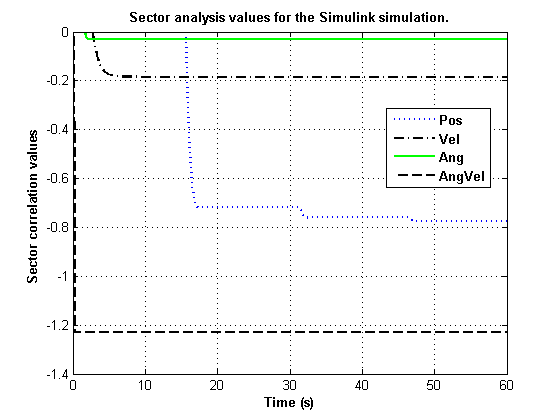
\includegraphics[width=0.85\columnwidth]{figures/simsectors}
    \caption{Sector search values for the simulated quad integrator example. }
    \label{fig:sectors1}
\end{figure}

\begin{figure}[htb]
\centering
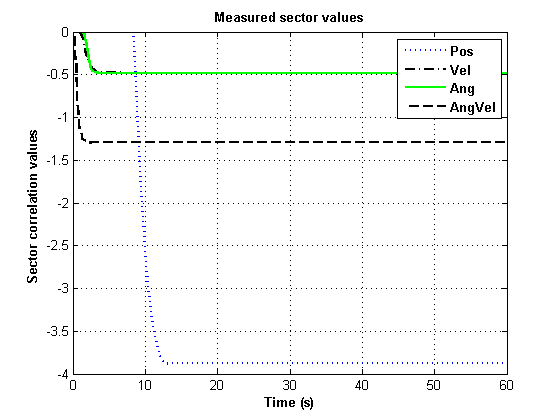
\includegraphics[width=0.85\columnwidth]{figures/meassectors}
    \caption{Sector search values for execution on the control platform
(including schedule effects). }
    \label{fig:sectors2}
\end{figure}

\begin{table*}[htb]
\centering

\begin{tabular}[width=0.85\columnwidth]{ | l | l | l | l | l | l | l | }

\hline
\textbf{Signal} & \textbf{Original Bound} & \textbf{Simulated Sector} & \textbf{Measured Sector} & \textbf{Delta} & \textbf{New Bound} & \textbf{New Sector} \\
\hline \hline
Angular Velocity & -1.333 & -1.2292 & -1.2963 & -0.0671 & -2.667 & -1.4568 \\
\hline
Angle & -0.5 & -0.0295 & -0.4831 & -0.4536 & -1.0 & -0.0068 \\
\hline
Velocity & -0.5 & -0.1856 & -0.4830 & -0.2974 & -1.0 &  -0.9324 \\
\hline
Position & -3.333 & -.7757 & -3.8811 & -3.1054 & -6.667 & -1.6081 \\
\hline
\end{tabular}
\caption{Sector value comparisons for simulation and execution on the actual platform.}
\label{tab:sectors}
\end{table*}

For this test we selected a square wave reference input near the highest frequency admissible by 
the controller.  Platform effects caused a significant deviation from our ideal sector estimates and 
bounds, as illustrated by the sector bound changes in Table \ref{tab:sectors}. For each digital 
control signal the table records the following (by column):
\begin{enumerate}
 \item Original Bound: the sector bound based on the original gain value ($-\frac{1}{k}$).
 \item Simulated Sector: the sector value recorded in simulation.
 \item Measured Sector: the initial sector value measured on the platform.
 \item Delta: the sector difference between the measured and simulated values.
 \item New Bound: the sector bound based on the newly adjusted gains.
 \item New Sector: the sector value measured on the platform with the new gains.
\end{enumerate}
Although the initial platform gains satisfied the sector stability conditions analytically and in 
simulation (comparing the Bound column tothe Simulated column in the table), the overall system 
response when deployed to the target platform resulted in significant position overshoot.  The 
measured sector value for position measured the farthest from the predicted value, and exceeded 
the gain bound for stability ($-1/k$), though no evidence of instability was visible in the 
plot of the output trajectory.  As all of the gains moved right up to the edge of 
their bounds when deployed, we adjusted all of the gains by $\frac{1}{2}$. Note that changing the 
gains changes the acceptable sector bound as well as the actual sector bounds themselves as shown 
in the table.  After adjusting the gains all of the sector values fell within the bounds.

On closer inspection we discovered
that the most significant platform effect was a non-ideal position gain condition for signals
with frequencies too close to the sampling rate.  Figs. \ref{fig:mags1} and 
\ref{fig:mags2} show a comparison of the ideal frequency response of the outer loop
controller block with an empirically measured frequency response for the same controller
block deployed on the target hardware.  The remedy was to add a simple input filter to 
cut off frequencies too close to the sampling rate. This effectively slows down the possible 
commands that can be issued to the system. The sector analysis blocks helped identify 
the position control component as the element whose behavior was farthest from predicted when 
deployed to the platform. 

\begin{figure}[htb]
\centering
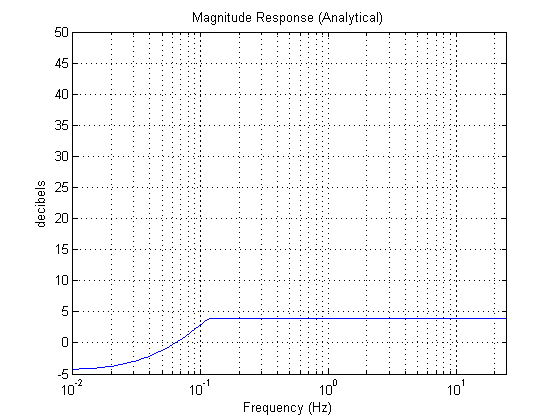
\includegraphics[width=\columnwidth]{figures/magresp_analytical}
    \caption{Magnitude frequency response (analytically predicted) for the quad integrator model.}
    \label{fig:mags1}
\end{figure}

\begin{figure}[htb]
\centering
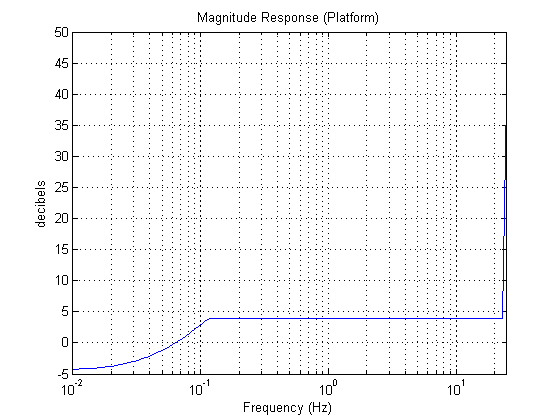
\includegraphics[width=\columnwidth]{figures/magresp_platform}
    \caption{Magnitude frequency response (measured) for the quad integrator model. Note the 
spike at the right-hand side of the plot.  This is a nonlinear gain anomaly due to the effects
of the saturation block, and which appears only for signals with frequencies right near the 
Nyquist sampling rate.}
    \label{fig:mags2}
\end{figure}

